\chapter{Tau Reconstruction and Identification in ATLAS}\label{ATLAS}
In this chapter, a review of the ATLAS detector at the Large Hadron Collider and a description of the reconstruction and identification of hadronic tau decays in ATLAS are presented.
\section{The LHC and the ATLAS experiment}
The Large Hadron Collider (LHC) is the largest particle accelerator currently operated by the European Organization for Nuclear Research (CERN). The LHC uses a 27 km tunnel where 2090, 15 m long, dipolar superconducting magnets bend the trajectories of two proton beams going in opposite directions. Each of the magnets is capable of producing a 8.33 T magnetic field and thus bending protons with an energy up to 7 TeV. The magnets are cooled down to 1.9 K in order to reach the superconducting state and the vacuum inside the beam pipes is of the order of $10^{-9}$ mbar. During LHC Run II, proton beams were accelerated to an energy of 6.5 TeV and they were collided in 4 interaction points where the detector experiments are located.

One of these experiments is the ATLAS (A Toroidal LHC ApparatuS) detector. It is a multi-purpose particle detector, capable of discovering new physics but also to perform high precision SM measurements. A complete description of the ATLAS detector design can be found at \cite{ATLAS:1999uwa}. ATLAS is a cylindrical detector composed by sub-detectors arranged in shells. The most inner layers are surrounded by a superconducting solenoid that generates a 2 T solenoidal magnetic field. ATLAS uses a right-handed coordinate system with its origin at the interaction point (IP) in the centre of the detector, the $z$-axis points along the beam pipe. The $x$-axis points towards the centre of the LHC ring and the $y$-axis in the vertical direction. The angle $\phi$ is defined in the $x-y$ plane and pseudorapidity is defined in terms of the polar angle $\theta$ as $\eta=-\log \tan(\theta/2)$. The angular distance is measured in units of $\Delta R\equiv \sqrt{(\Delta\phi)^2+(\Delta\eta)^2}$.

The most inner detector is responsible for track and vertex reconstruction and it consist of silicon pixel, silicon microstrip and transition radiation tracking detectors. The system has a coverage of $|\eta|<2.5$. The tracker system is followed by a lead/liquid-argon electromagnetic calorimeter (EC) and a steel/scintillator-tile hadron calorimeter (HC) that provide energy measurements with high granularity for electromagnetic showers and hadrons. The end-cap and forward EC and HC use LAr technology detectors and extend up to a $|\eta=4.9|$ region. The outermost detection system is a muon spectrometer (MS) that takes advantage of the bending power of a system of three air-core toroidal superconducting magnet systems.

Electrons are reconstructed matching a track in the inner tracking system and energy deposits in the EM calorimeter. Electrons have also different ID working points associated with them. More information on the electron reconstruction and ID can be find at \cite{Aaboud:2019ynx}. Muon reconstruction is as well independently done at the inner tracking detector and in the MS. Tracks in each subdetector are then matched and depending on different subdetector information and reconstruction algorithms muons are classified in different types \cite{Aad:2016jkr}. Hadronic jets are built from energy deposits in the calorimeters, using the anti-$k_t$ algorithm with radius parameter $R=0.4$ \cite{Cacciari:2008gp}. High-level tagging algorithms combine the outputs from different low-level algorithms in order to tag the flavour of the jets. In the case of bottom flavour jets (b-jets) the MV2 algorithm is used \cite{ATLAS:2017bcq}. It takes into account features like the impact parameter, which is the shortest distance between the primary vertex (PV) and the $z$-axis. The PV vertex is defined as the one having the highest sum of the squared transverse momenta of the tracks associated with the same vertex \cite{Aaboud:2016rmg,TheATLAScollaboration:2015hdc}. More information on the b-tagging algorithms can be find at \cite{Aad:2019aic}.
  
\section{Tau Reconstruction and Identification on the ATLAS detector}
Leptonically decaying taus ($\tau_\text{lep}$), may have a higher impact parameter and tend to have a softer $p_T$ spectrum compared with prompt muons or electrons coming from W or Z boson decays. In practice, the small differences in these variables make it difficult to differentiate between $\taul$ and prompt muons or electrons. In the case of hadronically decaying taus ($\tau_\text{had}$), as we will see, there are a lot more variables we could use to tag the presence of a $\tauh$.

As we saw in section \ref{chap2sec1}, $\tauh$ decays can be classified in 1-prong or 3-prong, depending on the number of charged particles in the decay. A detailed review of the reconstruction procedure for $\tauh$ is discussed in \cite{Aad:2014rga}. $\tauh$ candidates are seeded by jets using the anti-$k_t$ algorithm \cite{Cacciari:2008gp} with a distance parameter of 0.4. Jets are required to have $p_T>10$ GeV and $|\eta|<2.5$. Candidates between the barrel and forward calorimeter ($1.37<|\eta|<1.52$) are excluded due to poor instrumentation in this region.

The axis of the seed jet is defined by the energy-weighted barycentre of all clusters of calorimeter cells, called \textit{TopoClusters} \cite{Aad:2016upy}. The $\tauh$ vertex is selected as the one having the highest $p_T$ sum of all the tracks with $p_T>0.5$ GeV within a cone of $R=0.2$ around the seed jet axis. Tracks within a cone of $R=0.4$ are classified with a set of boosted decision trees (BDTs) into core and isolation tracks, the number of core tracks defines the number of prongs. Candidates with neither one or three tracks are rejected. Additionally, the sum of the charge of the tracks is required to be $\pm 1$.     

The tau reconstruction algorithm does not sufficient provide discrimination against jets that could mimic the signal of a $\tauh$ decay in the detector. Therefore, algorithms that perform this task have been developed. Previously, a BDT was used to discriminate jets against $\tauh$. Recently, a recurrent neural network (RNN) classifier that provides improved performance compared with the BDTs is used \cite{Deutsch:2680523}.

The RNN makes use of a set of variables like: $\tauh$ track features, information about energy deposits on the calorimeters clusters and high level features like the mass of the $\tauh$ candidate tracks. These variables are used to exploit the differences in the shapes of the showers between $\tauh$ and jets. In general, $\tauh$ showers tend to be more collimated and to have fewer tracks than jets. A representation of this is shown in Fig.\ref{Fig4}. 

\begin{figure}[htbp]
	\centering
	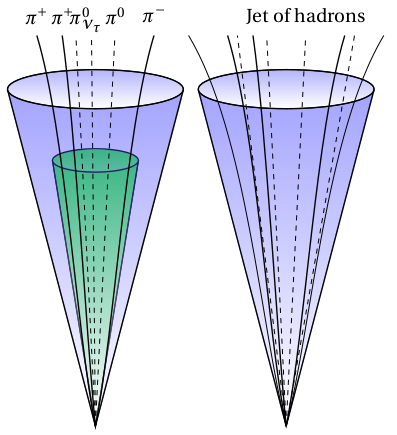
\includegraphics[width=0.4\textwidth]{figures/Fig4}
	\caption{Graphic representation that shows the main differences between a 3-prong $\tauh$ and a jet originated from quark or gluon radiation (QCD jets). Charged hadrons are shown as thick lines and dashed lines represent neutral particles. The green cone is drawn to depict how $\tauh$ product decays are more collimated. Taken from \cite{SamImage}.}
	\label{Fig4}
\end{figure}
Separate algorithms are trained for 1-prong and 3-prongs. The final RNN score assigned to each candidate corresponds to the fraction of rejected true $\tauh$, independent of $p_T$ and number of interactions per bunch crossing (pileup). Four working points with increasing background rejection are defined to be used in physics analysis. The working points and background rejection factors are shown in Table \ref{Table2}. A plot comparing the true $\tauh$ selection efficiency versus the background rejection power for the RNN and BDT algorithm is shown in Fig.\ref{Fig5}, the performance of the RNN is better than the BDT classifier. Finally, the distribution for the RNN score for true and fake $\tauh$ is shown in Fig.\ref{Fig6}, for both 1-prong and 3-prong decays.
\begin{table}[htbp]
	\centering
	\begin{tabular}{|l|l|l|l|l|l|l|}
		\hline
		Working point & \multicolumn{2}{l|}{Singal efficiency (\%)} & \multicolumn{2}{l|}{BG rejection BDT} & \multicolumn{2}{l|}{BG rejection RNN} \\ \hline
		& 1-prong              & 3-prong              & 1-prong               & 3-prong               & 1-prong               & 3-prong               \\ \hline
		Tight         & 60                   & 45                   & 40                    & 400                   & 70                    & 700                   \\ \hline
		Medium        & 75                   & 60                   & 20                    & 150                   & 35                    & 240                   \\ \hline
		Loose         & 85                   & 75                   & 12                    & 61                    & 21                    & 90                    \\ \hline
		Very loose    & 95                   & 95                   & 5.3                   & 11.2                  & 9.9                   & 16                    \\ \hline
	\end{tabular}
	\caption{Working points with their corresponding true $\tauh$ selection efficiency and the background rejection factors \cite{Deutsch:2680523}. The scores are shown for both RNN and BDT algorithms.}
	\label{Table2}
\end{table}
\begin{figure}[htbp]
	\centering
	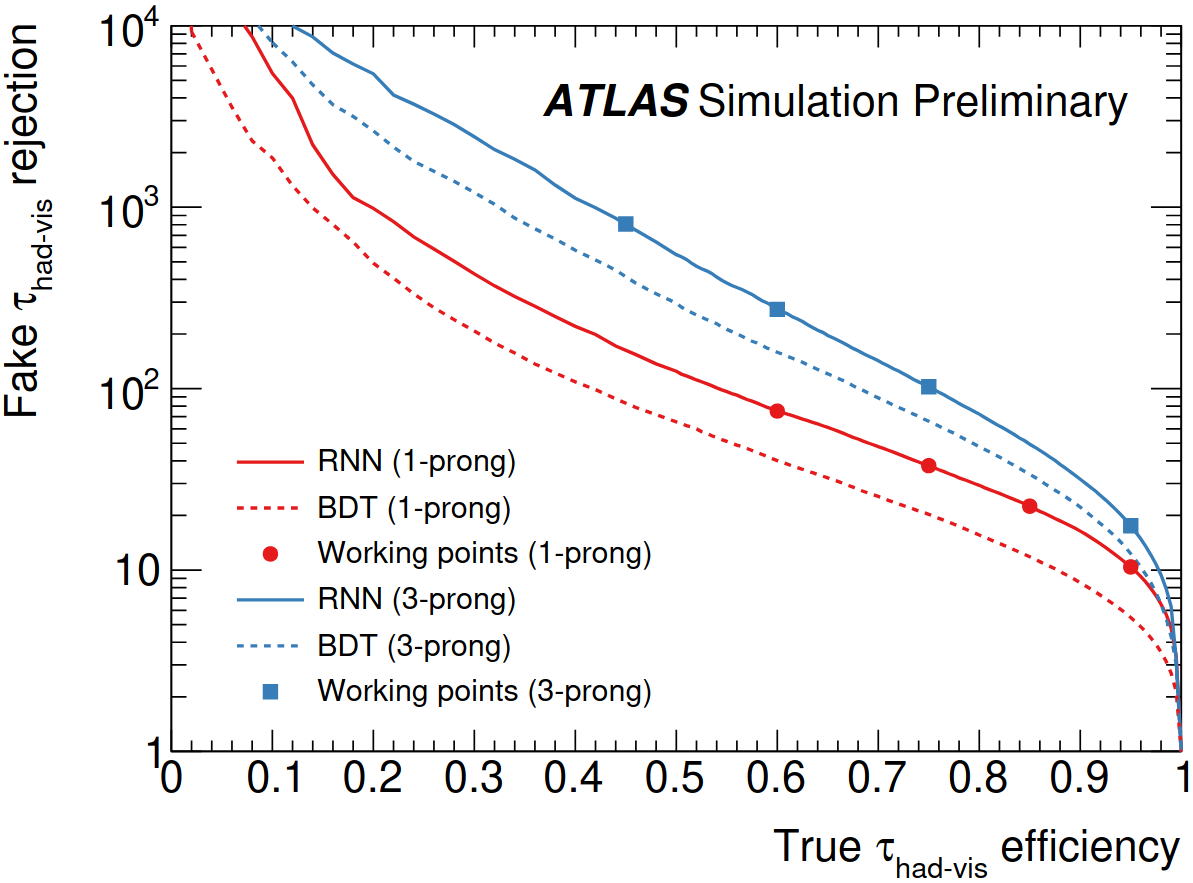
\includegraphics[width=0.5\textwidth]{figures/Fig5}
	\caption{Comparisson between the performance of BDT and RNN algorithms. Working points are shown as solid dots. Notice there is a trade off between true $\tauh$ efficiency and background rejection power. Taken from \cite{Deutsch:2680523}.}
	\label{Fig5}
\end{figure}
\begin{figure}[htbp]
	\centering
	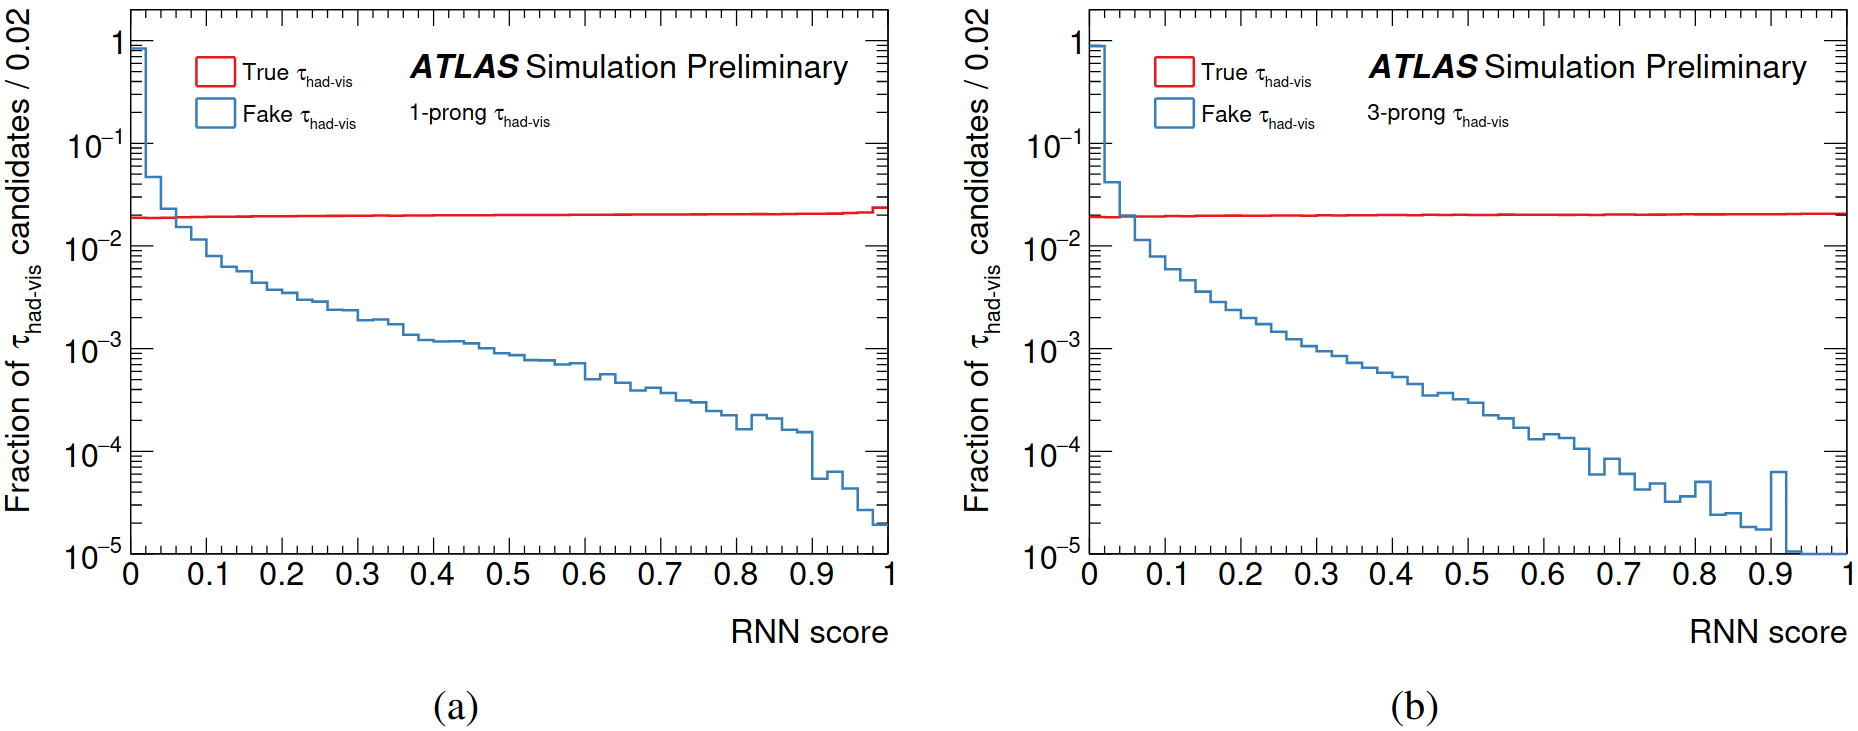
\includegraphics[width=1\textwidth]{figures/Fig6}
	\caption{Distribution of the RNN scores for true and fake $\tauh$ candidates for 1-prong (a) and 3-prong (b) cases. Taken from \cite{Deutsch:2680523}.}
	\label{Fig6}
\end{figure}